\chapter{Resultados y discusión}

En este capítulo se presentan los resultados más importantes de este trabajo,
tomando en cuenta los objetivos de esta tesis, sobre la partición de la energía
y la formación de los cúmulos de agua.

%%Separador 

\section{Bases y Métodos}

Las geometrías de los cúmulos diferentes a diez moléculas de agua fueron
tomados de la literatura~\cite{Toche2016, Yoo2010}.  En los casos de los
cúmulos con 10 moléculas de agua, las geometrías están basadas en la estructura
a adamantano. Donde los átomos de C fueron remplazados por O y los enlaces
covalentes C-C con EHs. De la diversificación de la distribución de los EHs se
obtuvieron cuatro estructuras. Posteriormente se agregaron moléculas a éstas
estructuras para tener, al menos, una molécula tetracoordinada.
%%El resto de cúmulos fueron tomados de la literatura~\cite{Toche2016,
%Yoo2010}.

Inicialmente se realizaron optimizaciones con el método HF/3-21G, para
garantizar que se trataban de mínimos locales, posteriormente se realizaron
optimizaciones HF/6-311\-+\-+\-G\-(d,\-p), MP2/aug-cc-pVTZ y
M06-2X/6-311++G(d,p), para elegir el método más favorable para la optimización,
el cual resultó ser M06-2X/6-311++G(d,p).  La elección del método se fundamenta
en que los métodos usados son variacionales, y como se señaló en la
metodología, el valor exacto representa una cota inferior para el cálculo, por
lo que los valores de energía obtenidas son comparables entre sí. A pesar de
que M06-2X no es \SI{100}{\percent} variacional y es posible estar
sobreestimando la energía del sistema, usar MP2 es bastante más caro
computacionalmente, además de que los valores no difieren significativamente de
aquellos obtenidos con M06-2X, como se muestra en la Figura \ref{HF_m062x}, por
lo que se optó por usar M06-2X para las optimizaciones.

\begin{figure}
    \centering
    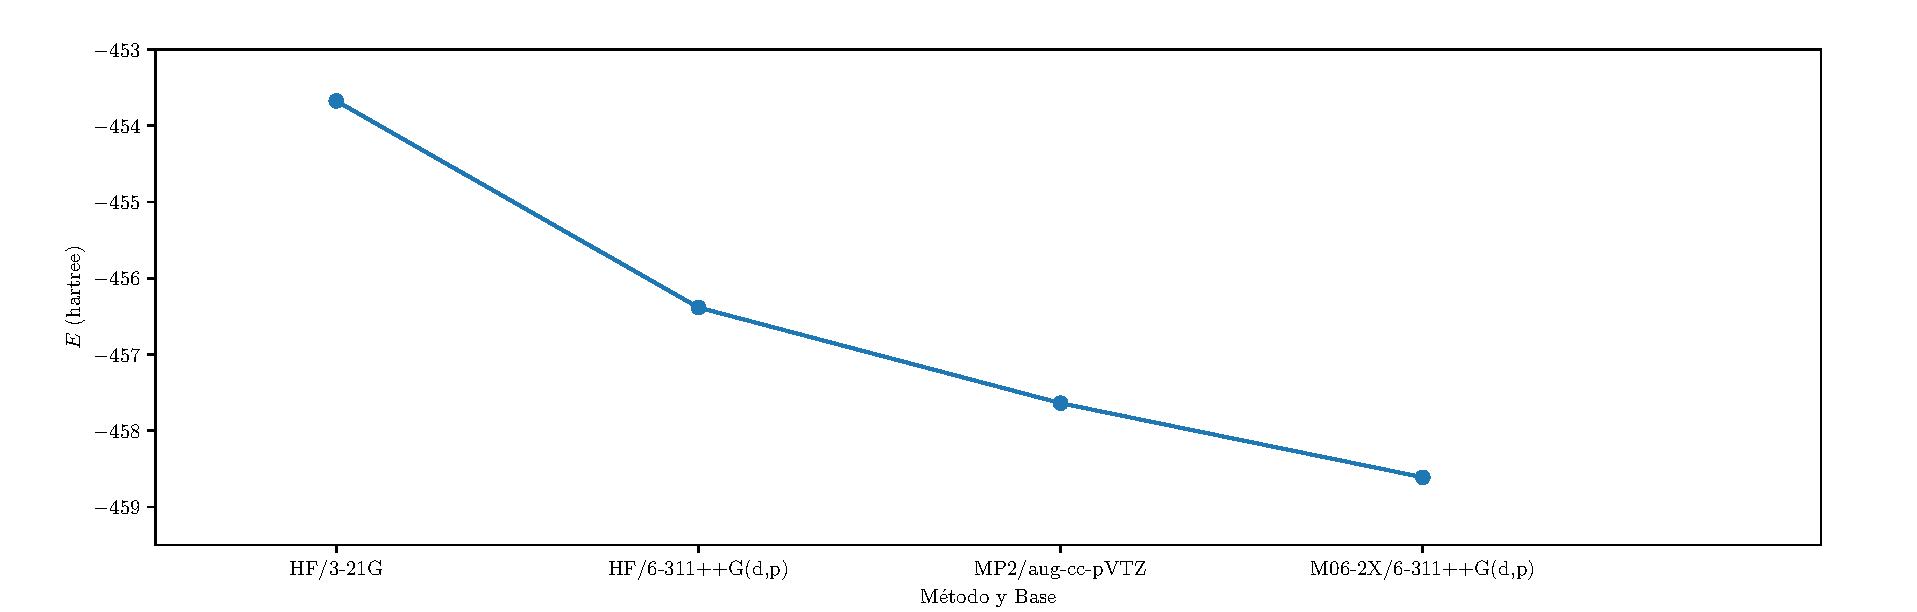
\includegraphics[width=1\textwidth]{4/graf/bases_f}
    \caption{Comparación de la energía calculada con las combinaciones
de métodos y bases.}
\label{HF_m062x}
\end{figure}

Una vez que se encontraron los mínimos locales en los cúmulos de agua, se
descartaron aquellos cuya energía fuera al menos \SI{5.0}{\kilo \calorie \per
\mole} mayor que la energía del cúmulo, con el mismo número de moléculas, de
menor energía. Esto porque, como se muestra en~\citenum{Yoo2010}, la abundancia
estadística de dichos cúmulos es despreciable en una distribución
Maxwell-Boltzmann, es decir, sus resultados no son representativos del
comportamiento de la mayoría. Los cúmulos descartados, por rebasar el límite de
las \SI{5.0}{\kilo \calorie \per \mole}, se encuentran en la Figura
\ref{descartados}, mientras que los cúmulos con los que se siguió trabajando
están en la Figura \ref{cumulos}.

\begin{figure}
    \centering
    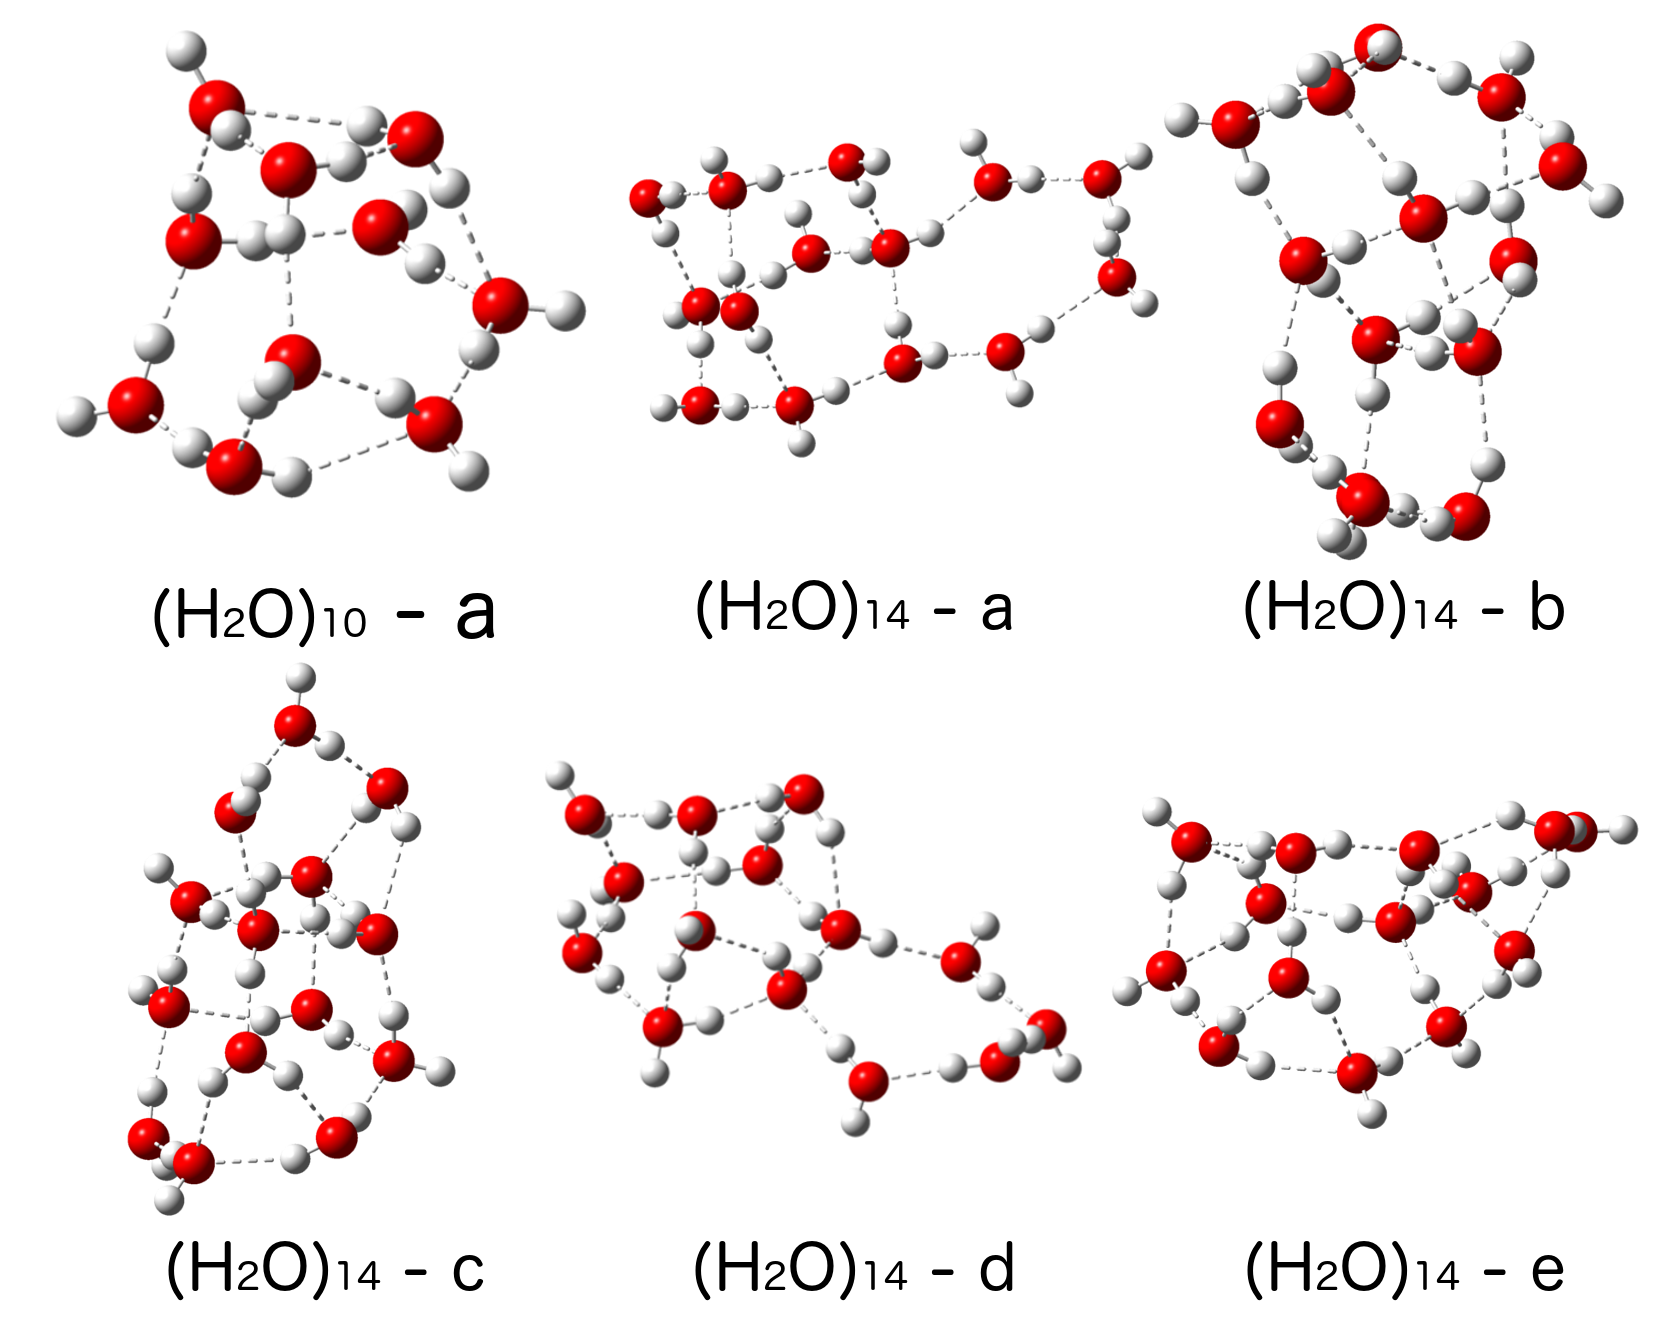
\includegraphics[width=0.60\textwidth]{4/img/descartados}
    \caption{Cúmulos descartados.}
\label{descartados}
\end{figure}
%
\begin{figure}
    \centering
    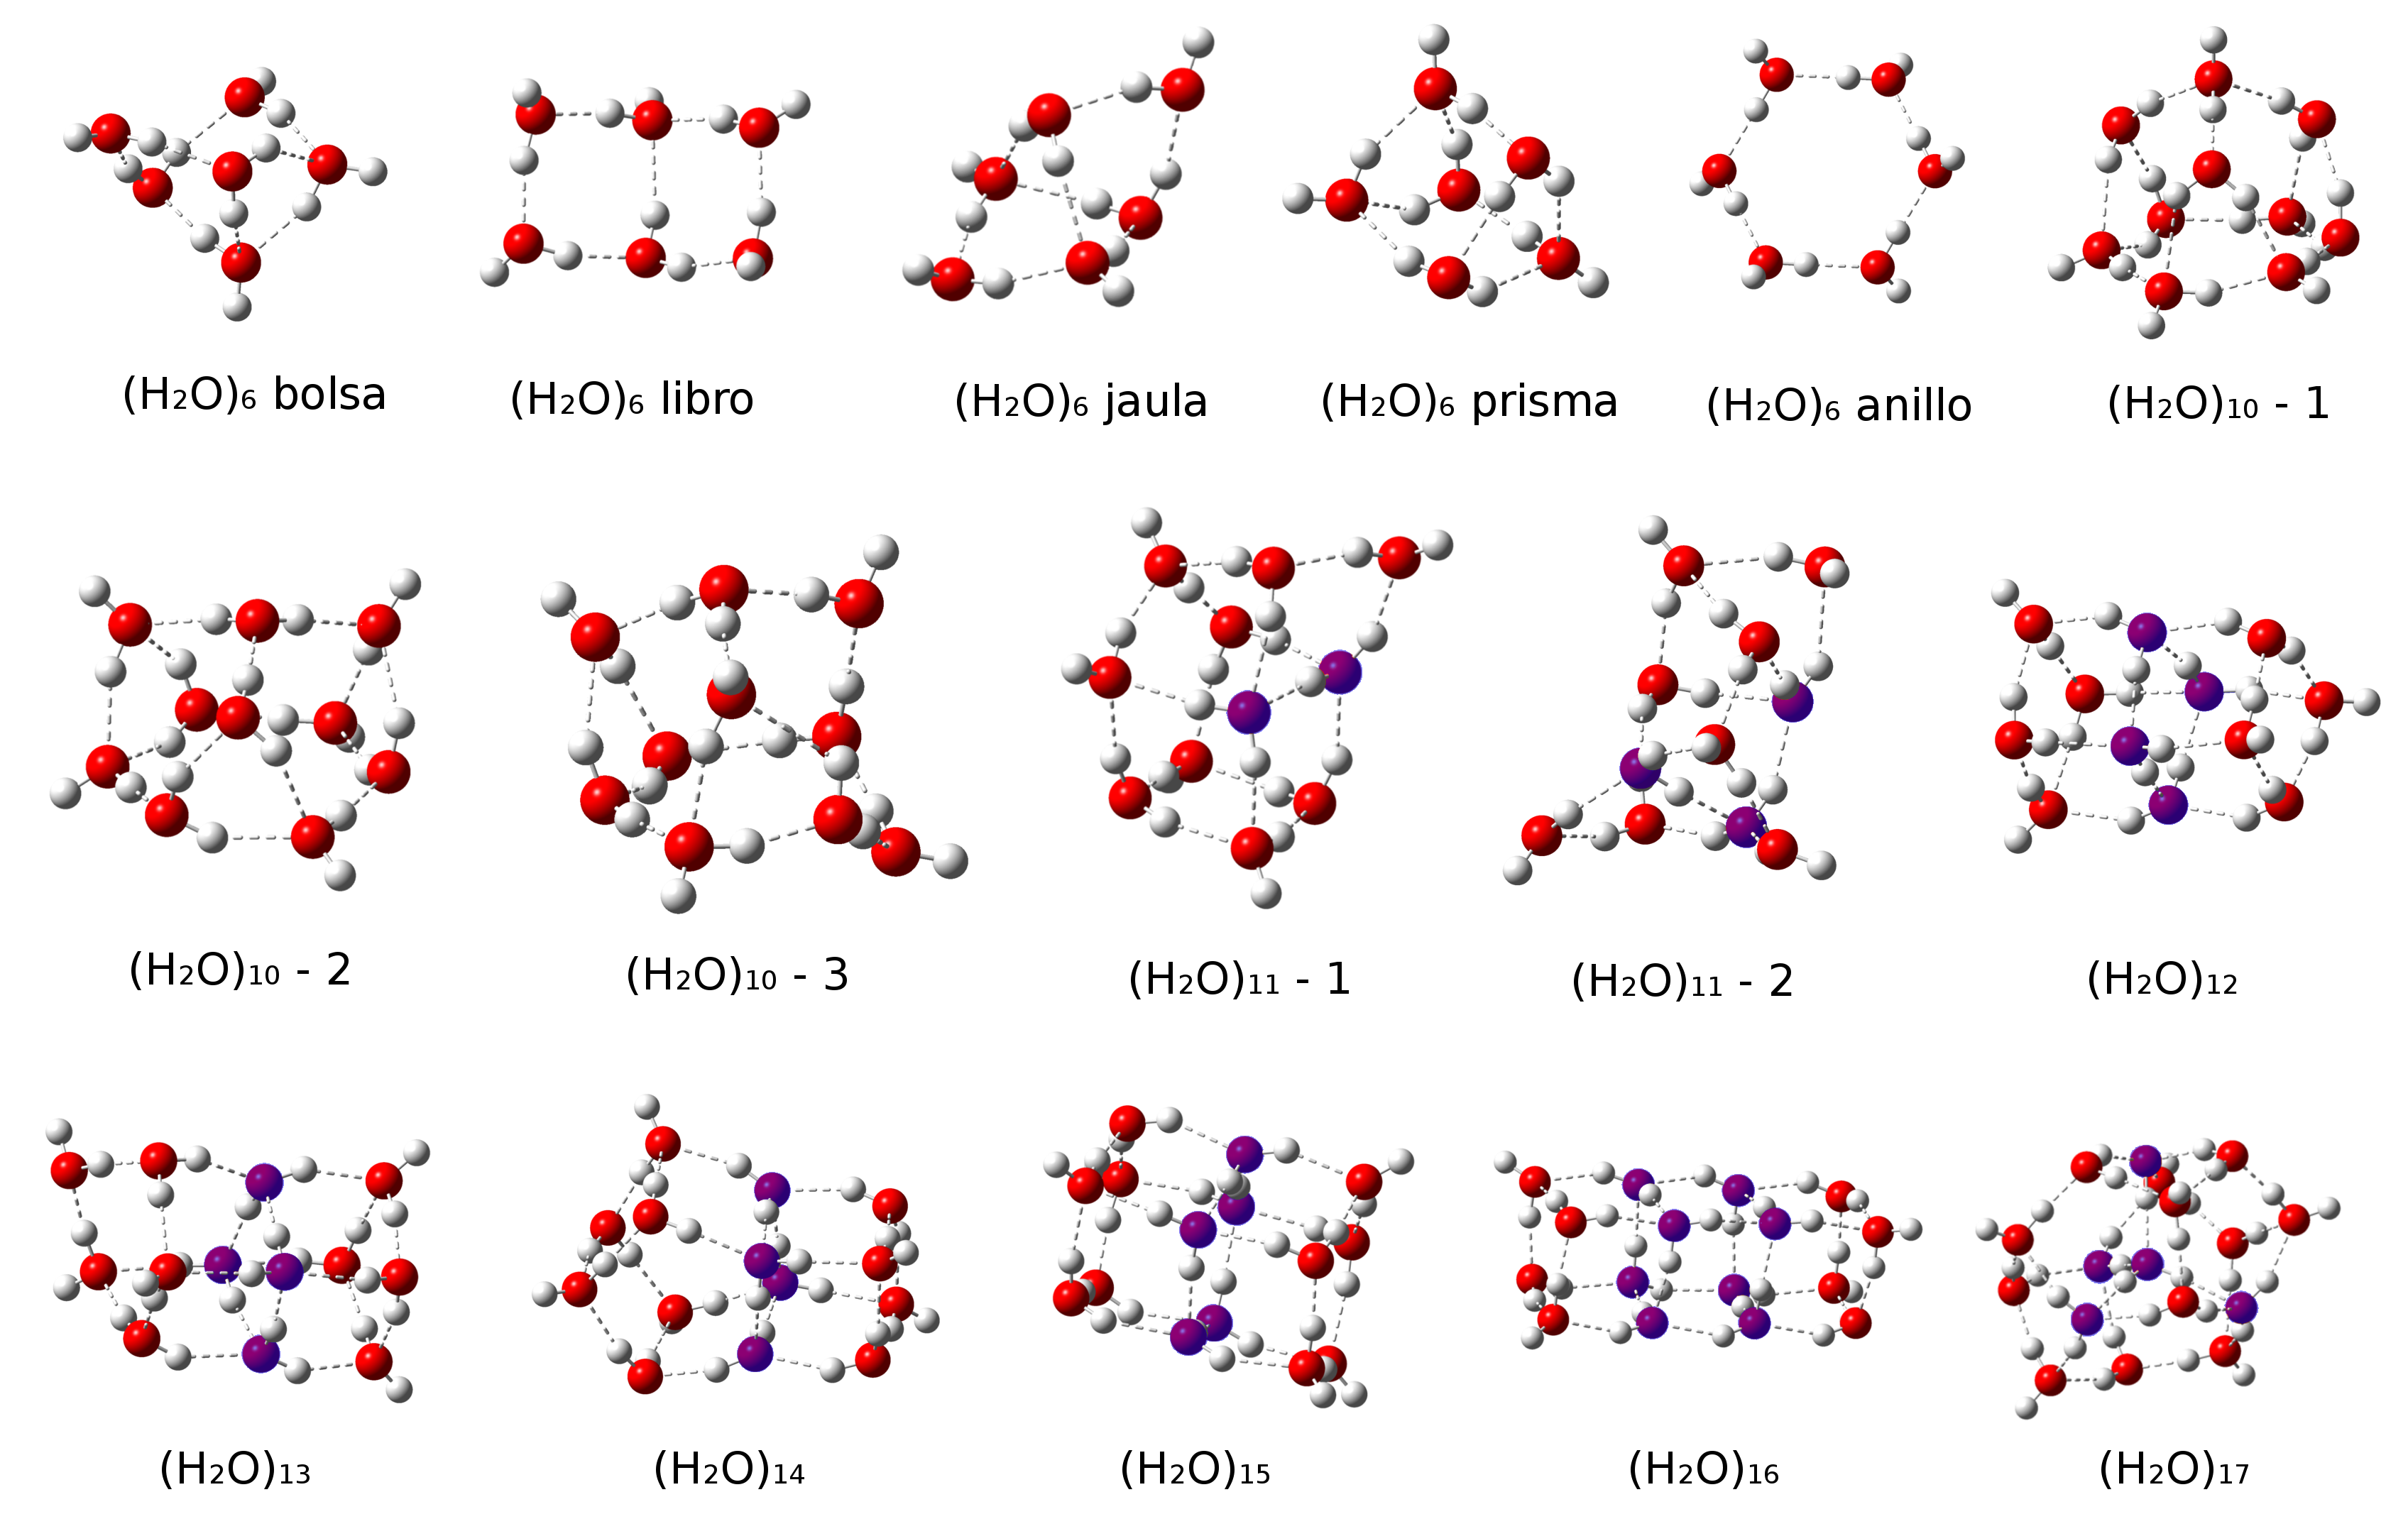
\includegraphics[width=1.00\textwidth]{4/img/cumulos}
    \caption{Cúmulos trabajados, los átomos de oxígeno marcados con tono azul
son parte de moléculas de agua tetracoordinadas.}
\label{cumulos}
\end{figure}

\section{Nueva Escala}

En la Tabla \ref{motivacion}~\cite{Toche2016} se muestra una propuesta de la
jerárquica de los EH entre moléculas de agua basada en su conectividad. Esta
escala se encuentra incompleta al no contemplar el caso de moléculas de agua
tetracoordinadas en los cúmulos. Considerando los sistemas presentados en la
Figura \ref{cumulos} podemos corregir esa omisión. En la Tabla \ref{scale2020}
se da una descripción de diez categorías de diferentes tipos de EHs. Además son
comparadas con la clasificación existente antes de contemplar el caso
tetracoordinado como se observa en la Figura \ref{2016_vs_2020}.

Los tipos de EHs descritos en la Tabla \ref{scale2020} están ordenadas de la
menos energética (1) a la más energética (10), con valores asociados a los
promedios de la energía de interacción entre los pares de moléculas presentados
en la Figura \ref{cumulos}. Como podemos observar el intervalo de las energías
de interacción es de \SI{-5}{\kilo \calorie \per \mole} a \SI{-10}{\kilo
\calorie \per \mole}. Si comparamos este  intervalo con la energía del dimero,
al mismo nivel de teoría que es de \SI{-6.6}{\kilo \calorie \per \mole}, vemos
que se puede favorecer la energía de interacción hasta un \SI{50}{\percent}.


\begin{table}[htbp]
  \begin{center}
    \caption{Jerarquía de los EH en cúmulos de agua presentados en esta tesis.}
    \begin{tabular}{c||p{12.5cm}}
      Tipo de EH & Descripción \\ \hline\hline
      1 & ($i$) El átomo de H involucrado en el EH proviene de un doble donador de EH
          y ($ii$) el oxígeno que participa en la interacción actúa como un doble aceptor.\\ \hline
      2 & Una molécula tetracoordinada interactúa como ($i$) donante de EH a una molécula
          tricoordinada que es doble aceptora o ($ii$) aceptora de EH de una molécula tricoordinada
          que es doble donadora. \\ \hline
      3 & Una molécula tetracoordinada interactúa con una dicoordinada ya sea donador
          o aceptor sencilla. \\ \hline
      4 & ($i$) El H de un doble donador de EH está enlazado con un oxígeno de un aceptor
          sencillo de EH o ($ii$) un oxígeno de un doble aceptor interactúa con un H
          de un donador sencillo. \\ \hline
      5 & Un enlace de hidrógeno es formado entre dos dobles donadores
          de EH o dos dobles aceptores de EH. \\ \hline
      6 & Las dos moléculas de agua involucradas son tetracoordinadas.\\ \hline
      7 & Una molécula tetracoordinada ($i$) dona EH a una doble
          donadora o ($ii$) acepta EH de una doble aceptora. \\ \hline
      8 & Un H de un donador sencillo de EH está enlazado con un oxígeno
          de un aceptor sencillo de EH. \\ \hline
      9 & ($i$) un hidrógeno de un doble aceptor de EH interactúa con el oxígeno
          de un donador sencillo o ($ii$) el oxígeno de un doble donador de EH
          interactúa con un hidrógeno de un sencillo aceptor. \\ \hline
      10 & El oxígeno de un doble donador de EH interactúa con un H de 
          un doble aceptor de EH. \\ 
    \end{tabular}
    \label{scale2020}
  \end{center}
\end{table}

\begin{wrapfigure}{l}{0.60\textwidth}
    \centering
    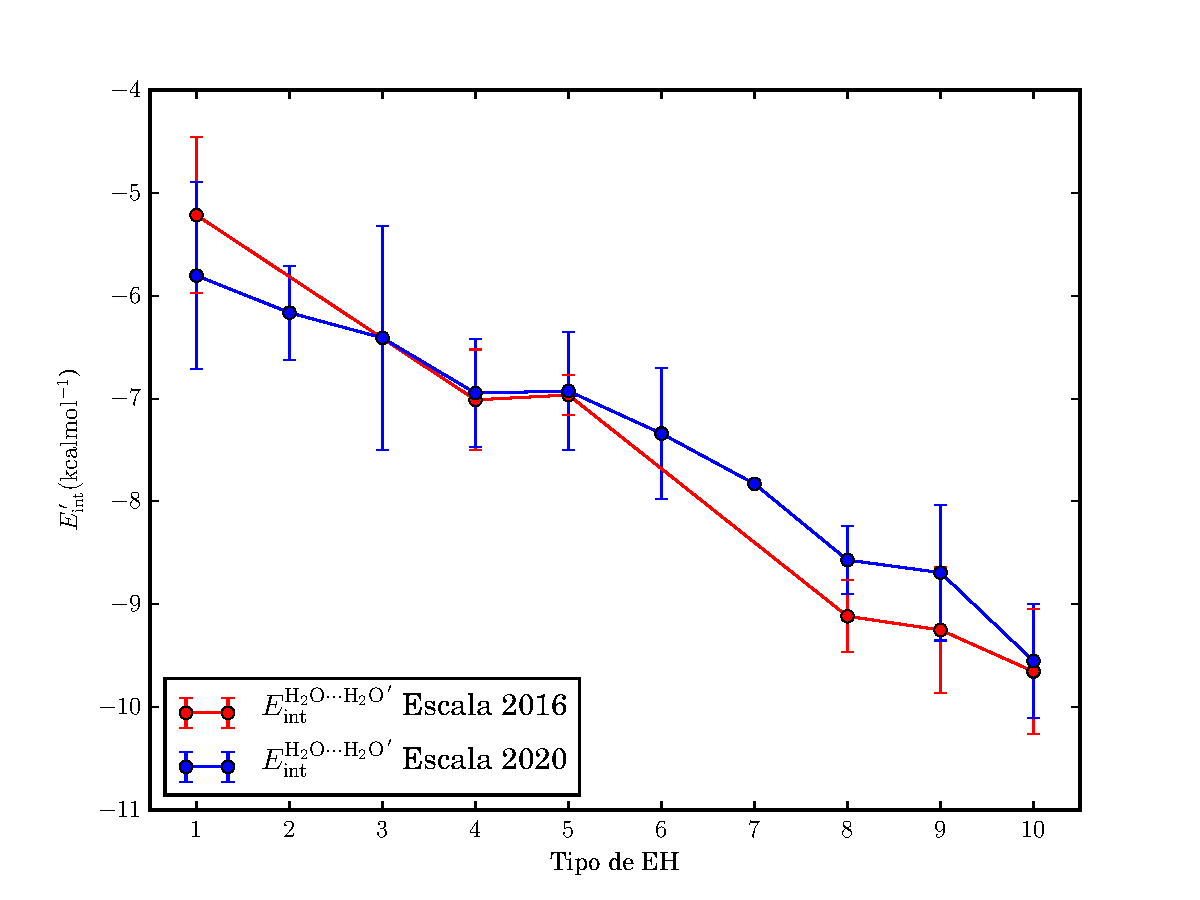
\includegraphics[width=0.65\textwidth]{4/img/New_vs_old_barraerror}
    \caption{Escala 2016 y 2020.}
\label{2016_vs_2020}
\end{wrapfigure}

En la Figura \ref{2016_vs_2020}, se presenta una comparación entre las escalas
obtenidas en 2016 por~\citenum{Toche2016} en rojo, la cual fue obtenida con la
aproximación MP2, y la obtenida en este trabajo en azul, calculada con el
formalismo de DFT y el funcional M06-2X. Estas escalas muestran la energía de
formación de un EH en función del tipo de enlace de hidrógeno, cabe señalar
que, a pesar de la diferencia en las metodologías, estas se encuentran en gran
concordancia. La razón de la pequeña diferencia entre las escales es que estas
energías son robustas ante el cambio de nivel de
teoría~\cite{JimenezGravalos2019}.

En la Figura \ref{2016_vs_2020} se muestra la interacción entre dos moléculas
tetracoordinadas, EH tipo (6), el cual está en medio de la escala. Con esto
podemos decir que la tetracoordinación está cerca de lo que consideramos como
un promedio total entre las interacciones analizadas. Otras categorías con
tetracoordinación son (2), (3) y (7). Las primeras dos son interacciones donde
la otra molécula es débil aceptor o donador débil, mientras que el último es
una interacción con una molécula que tiene una mayor disposición para formar un
EH. El EH más débil encontrado, el tipo (1), está asociado con la
in\-te\-rac\-ción entre un donador de hidrógeno, que es un doble donador, y una
molécula aceptora que toma el papel de un doble aceptor de hidrógeno. Por otro
lado el EH más fuerte, el tipo (10), se da entre una molécula doble aceptora
que toma el papel de donadora, para formar un tercer EH, con una molécula doble
donadora que funge de aceptora. 
%
%
%Finalmente en el caso más débil (el tipo 1) y el más fuerte (el tipo 10), el
%EH está formado exclusivamente por moléculas de agua con una topología
%contraria para formar un EH extra, en el caso de los primeros, o a favor en el
%caso de los últimos.
%

\begin{wrapfigure}[16]{r}{0.60\textwidth}
    \centering
    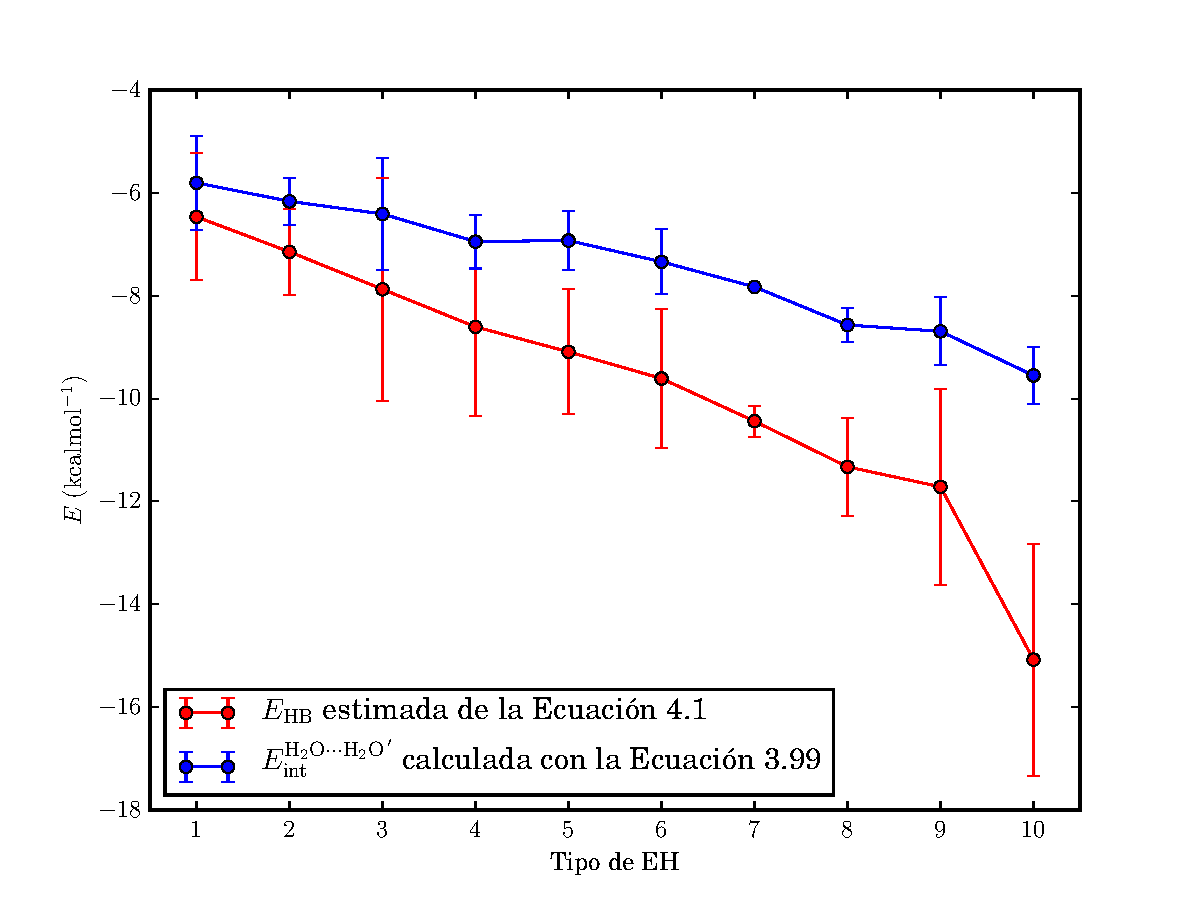
\includegraphics[width=0.65\textwidth]{4/img/EHB_vs_Eint}
    \caption{Energía estimada para EH~\cite{Espinosa1998} vs. energía de interacción.}
\label{estimada}
\end{wrapfigure}

Espinosa y colaboradores propusieron en~\citenum{Espinosa1998} que es posible
aproximar la energía de formación de un EH utilizando como función la densidad
de energía potencial en el punto crítico de enlace
$\mathrm{V(\mathbf{r}_{bcp})}$,
%
\begin{align}
\mathrm{E_{HB}}\approx 0.5\mathrm{V(\mathbf{r}_{bcp})}.
\label{estimada_eq}
\end{align}
%
%\noindent donde $\mathbf{r}_{bcp}$ es la posición del punto crítico asociado al EH, y
%V la densidad de energía potencial en el punto crítico.

La Figura \ref{estimada} muestra los valores correspondientes a esta
estimación, y los compara con los valores de interacción entre grupos
${E_{\mathrm{int}}^{\mathrm{H_2O}\cdots\mathrm{H_2O}^{ \, \prime}}}$. Como se
puede apreciar, en todos los casos la energía estimada es mayor que la
calculada con la metodología IQA. A pesar de  que las diferencias se vuelven
más pronunciadas a medida que el EH se vuelve más energético, las tendencias de
ambas funciones son decrecientes con respecto a la variable categórica del tipo
de enlace de hidrógeno, es decir, guardan la misma tendencia.

\section{Transferencia de Carga en Enlaces de Hidrógeno}

Ambas jerarquías de los EH, la sugerida en esta tesis y la que se presenta
en~\citenum{Toche2016}, pueden racionalizarse en términos de la transferencia
de carga que ocurre en la formación de un EH. La formación de un enlace de
hidrógeno dentro de un cúmulo de agua, se puede considerar como una reacción
ácido-base de Lewis, es decir una transferencia de electrones desde el aceptor
del átomo de hidrógeno al donador en el EH. Tal transferencia de carga facilita
tanto $i$) la capacidad de donar un átomo de hidrógeno de la molécula aceptora
del primer EH, ya que ahora tiene un déficit de carga, y $ii$) la capacidad de
aceptar un hidrógeno del fragmento donador del primer EH, ya que su átomo de
oxígeno es más rico en electrones que en una molécula de agua aislada. Estos
argumentos se muestran en la Figura \ref{transferencia_2}.

\begin{figure}[hb]%{l}{0.45\textwidth}
    \centering
    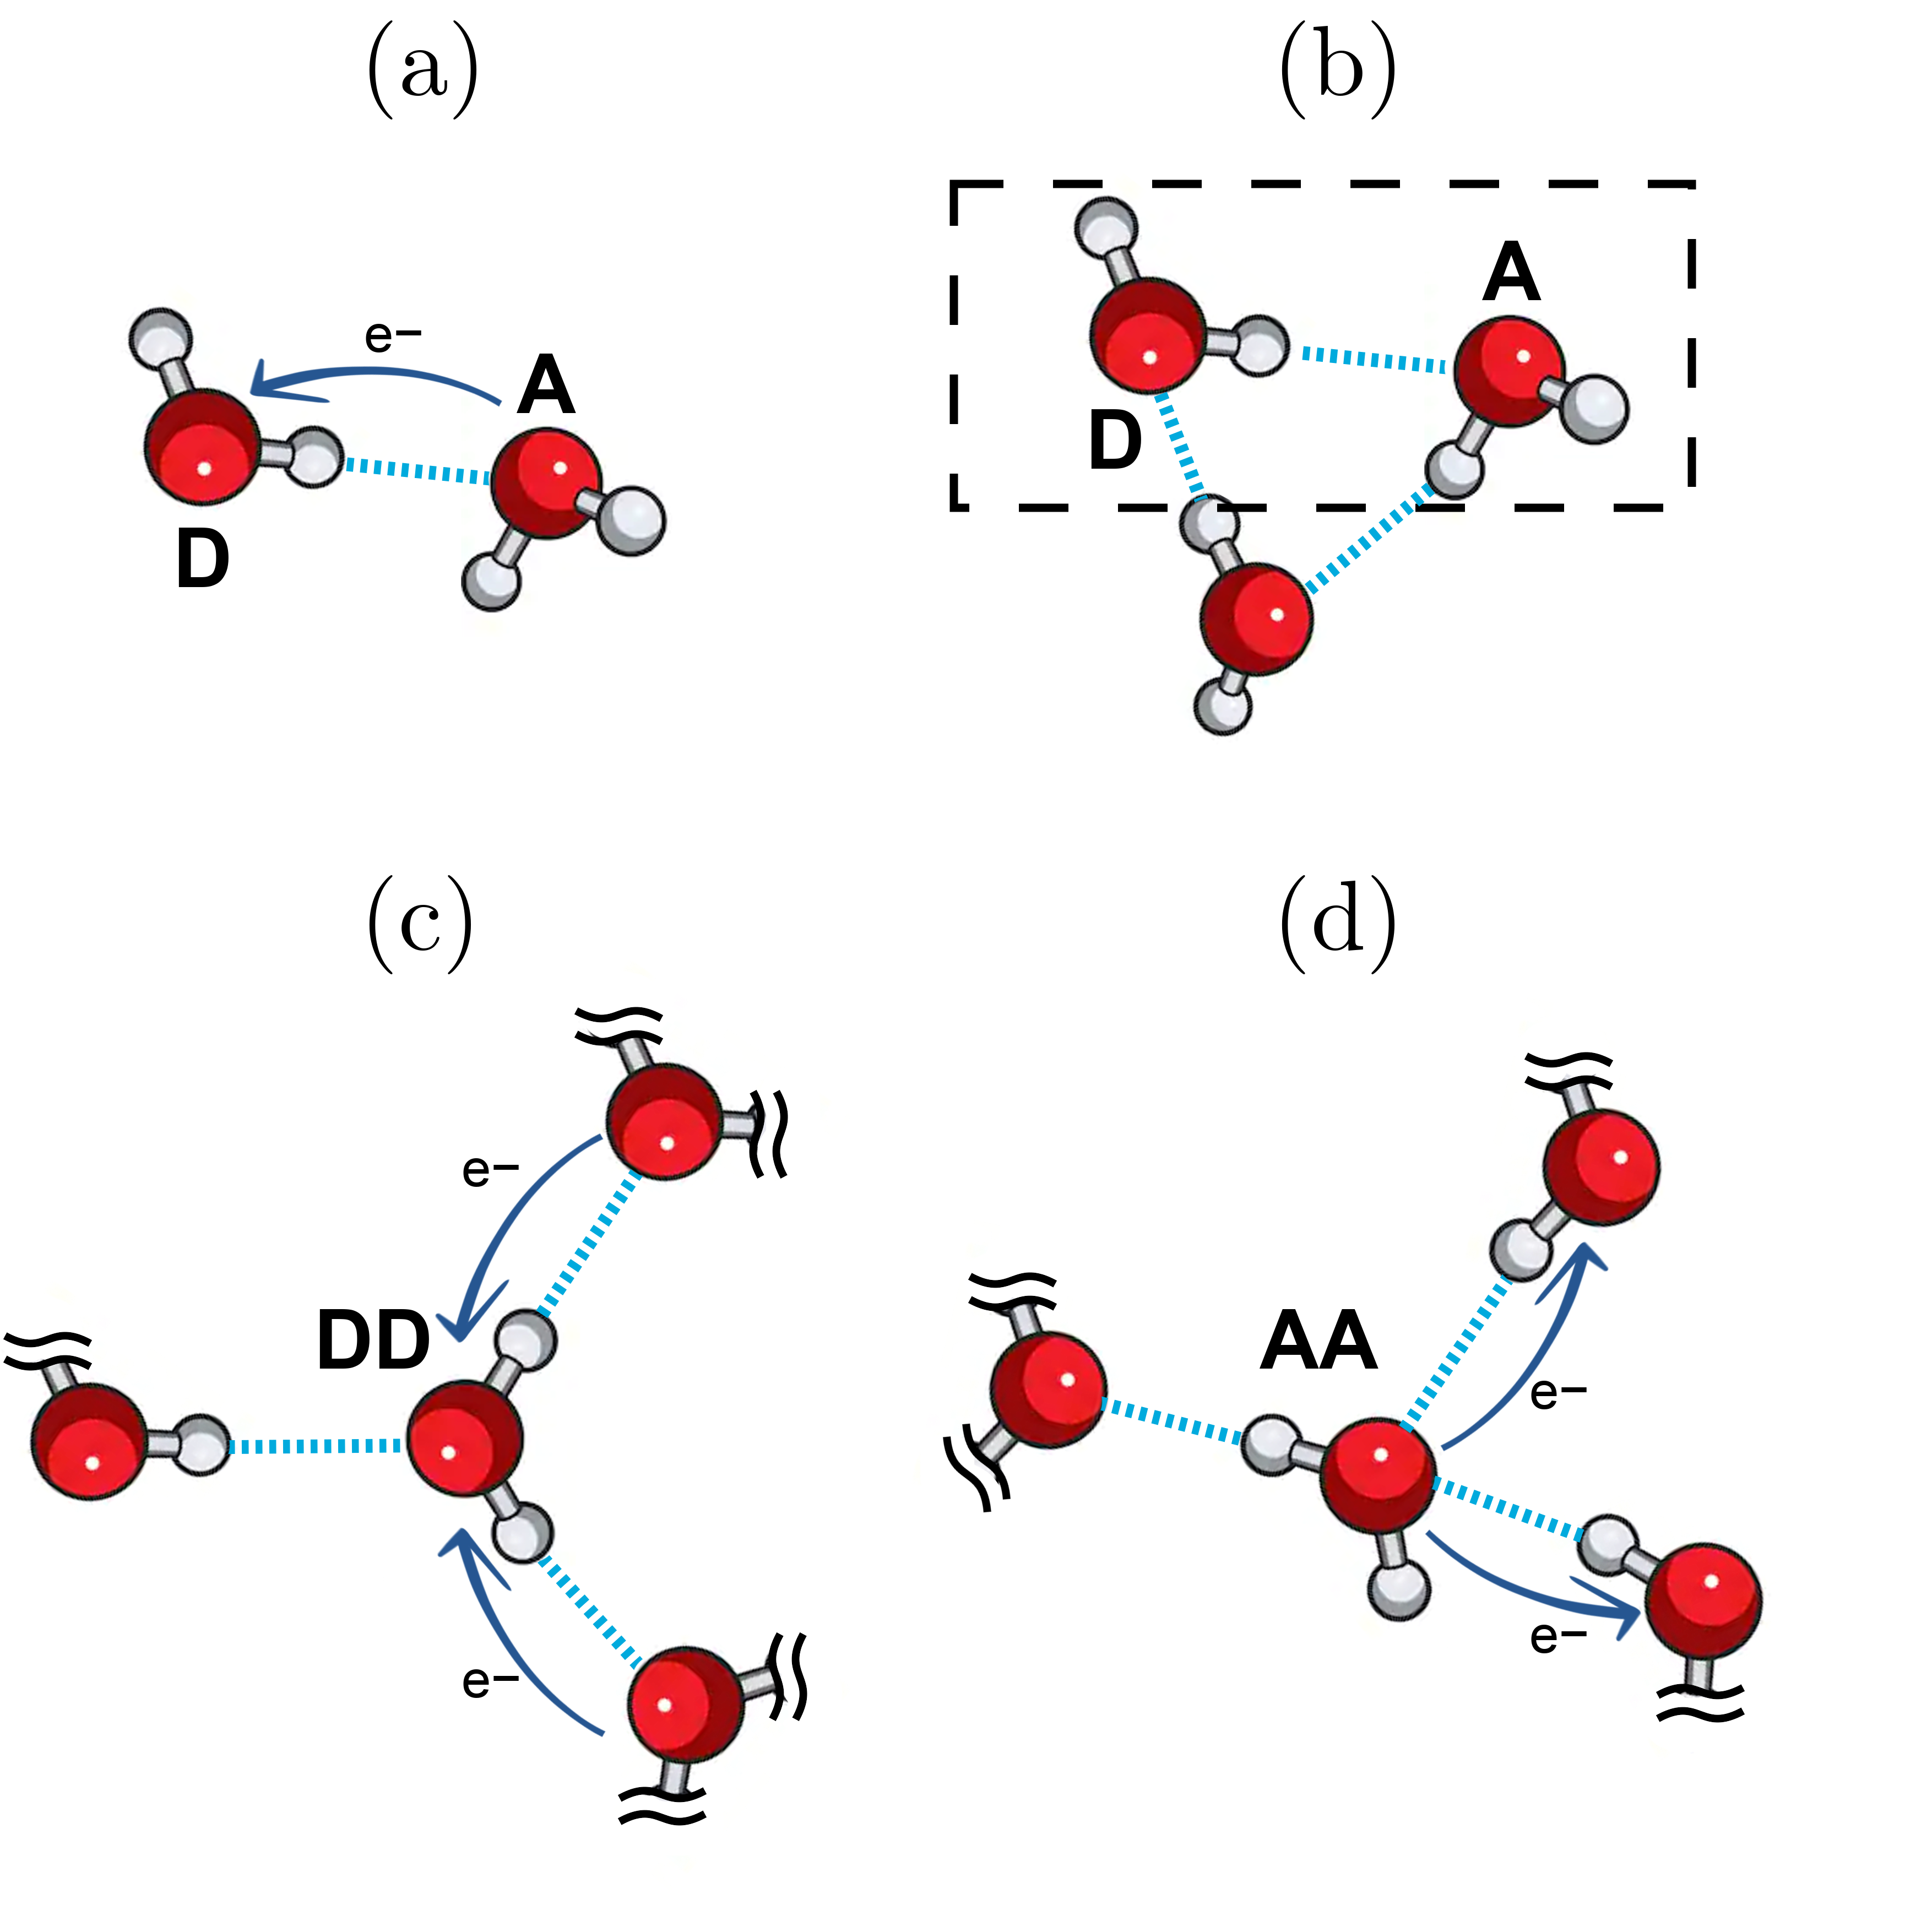
\includegraphics[width=0.67\textwidth]{4/img/figura5}
    \caption{Transferencia de densidad electrónica en los diferentes arreglos dentro de los cúmulos de agua aquí estudiados.}
\label{transferencia_2}
\end{figure}

Estos efectos dan paso a la cooperatividad de enlaces de hidrógeno, observable
por ejemplo en los cúmulos cíclicos homodrómicos (Figura \ref{transferencia_2}
(b)), como de anticooperatividad~\cite{steiner}. En la Figura
\ref{transferencia_2} (c) se muestra un doble donador de EH tricoordinado,
donde estos enlaces se debilitan entre sí, pero además ambas transferencias de
carga contribuyen a que el átomo de oxígeno sea un mejor aceptor de EH. Este
efecto refuerza al EH en la parte izquierda de la Figura \ref{transferencia_2}
(c), por lo que uno puede considerar que los donantes dobles de EH son malos
donadores, pero buenos aceptores de EH. Siguiendo con argumentos similares
sobre la transferencia de carga relacionada a los EHs es posible llegar a la
conclusión de que los EHs en la parte derecha de la Figura
\ref{transferencia_2} (d), presentan efectos anticooperativos y que los
hidrógenos de una molécula de agua, que es doble aceptora, son más ácidos que
los del agua aislada, por lo cual, debería formar EHs más fuertes que los
presentes en el dimero de agua, es decir, los dobles donadores de EH son
comparativamente donantes débiles, pero buenos aceptores de EH.  Por lo tanto,
el tipo de enlace más débil de EH en la jerarquía sugerida en esta tesis
involucra: $i$) un donante doble de EH que actúa como el donante de EH y $ii$)
un doble aceptor de EH que funciona como el aceptor de EH en la interacción.

Por otro lado, el EH más fuerte en la escala es entre un doble donador de EH
actuando como aceptor de EH y un doble aceptor actuando como el donador de EH,
como se ilustra en la Figura \ref{img6} (f). En el caso del agua
tetracoordinada, al ser tanto doble donadora como doble aceptora
simultáneamente, es difícil clasificarla en términos comparativos como una
buena o mala donadora o aceptora. Por el contrario, es posible clasificar al
agua dicoordinada, como buena donadora o aceptora en función de si actúa como
donadora o aceptora en el primer EH.  Además, la Figura \ref{img6} (b) muestra
que el tipo más débil de EH para moléculas de agua tetracoordinadas involucra a
donantes o aceptores de EHs pobres.  De forma análoga, los EHs más fuertes
formados por monómeros de agua tetracoordinados son resultado de interacciones
con los mejores donantes o aceptores de EH como se muestra en la Figura
\ref{img6} (e). Las Figuras \ref{img6} (c) y \ref{img6} (d) representan
situaciones que son intermedias entre estos dos extremos.

\begin{figure}%{l}{0.45\textwidth}
    \centering
    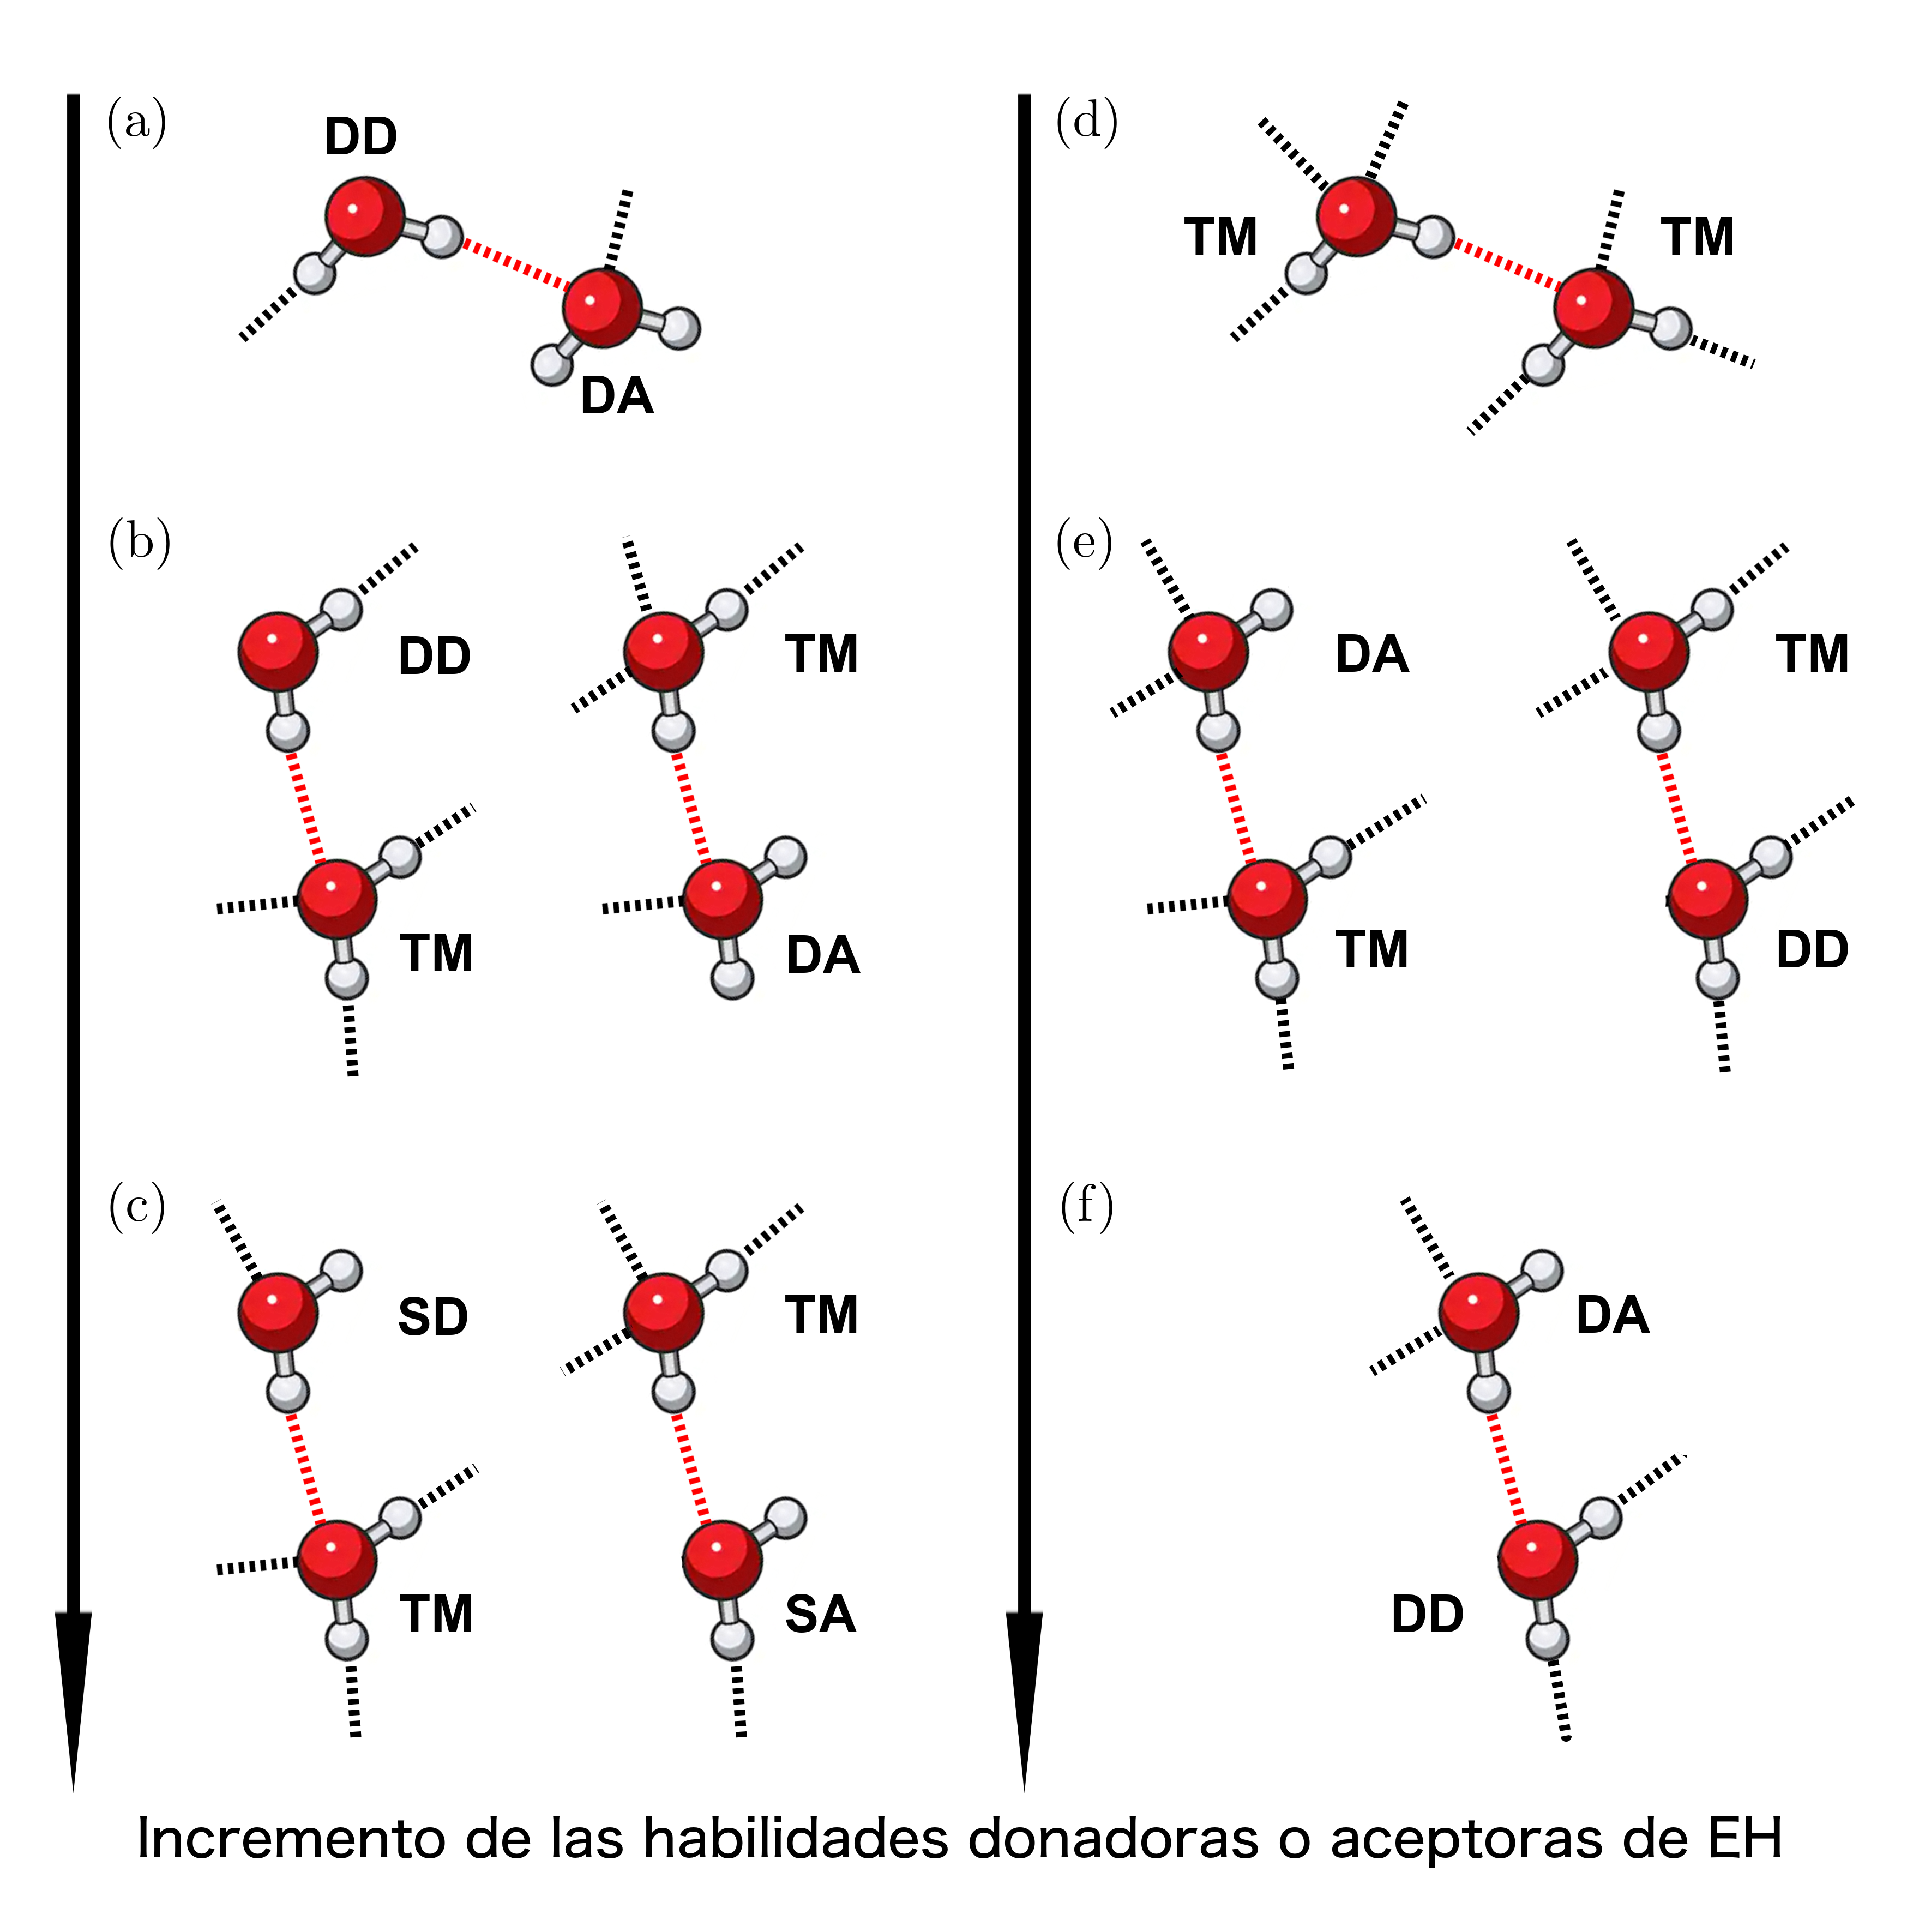
\includegraphics[width=1.00\textwidth]{4/img/figure6}
    \caption{\textbf{DA}=Doble Aceptor de EH, \textbf{DD}=Doble Donador de EH, \textbf{TM}=Monómero Tetracoordinado, \textbf{SA}=Aceptor Sencillo de EH, \textbf{SD}=Donador Sencillo de EH.}
\label{img6}
\end{figure}

La Figura \ref{transicion_} muestra la transición, desde la interacción
considerada como el EH más fuerte, hasta aquella que se da entre dos moléculas
tetracoordinadas pasando por la interacción de una molécula tricoordinada con
una tetracoordinada. Esto proporciona información valiosa sobre los efectos de
la formación de arreglos que involucran  moléculas tetracoordinadas en cúmulos
de H$_2$O. Primero, cuando el donador \textbf{D} de EH en la parte izquierda de
la Figura \ref{transicion_} se convierte en una molécula tetracoordinada, se
convierte en $i$) un peor donante y $ii$) un mejor aceptor de EH. El primer
hecho debilita al EH indicado en color rojo en la Figura \ref{transicion_},
pero el segundo fortalece a los EHs de la molécula \textbf{D} marcados con la
letra $m$. Del mismo modo, cuando el cuarto EH se forma en la molécula
$\mathbf{A}$, esta molécula se convierte en $i$) un peor aceptor y $ii$) un
mejor donador de EH. Estos resultados tienen efectos similares en la fuerza de
los EHs donde la molécula $\mathbf{A}$ está involucrada, es decir, el EH
indicado en rojo en la Figura \ref{transicion_} se debilita aún más y los otros
EHs de $\mathbf{A}$ se vuelven más fuertes (aquellos marcados con la letra
$w$).  En general, la tetracoordinación genera un debilitamiento de los EH que
se ve compensado por el mayor número de enlaces formados dentro del cúmulo.
%
\begin{figure}%{l}{0.45\textwidth}
    \centering
    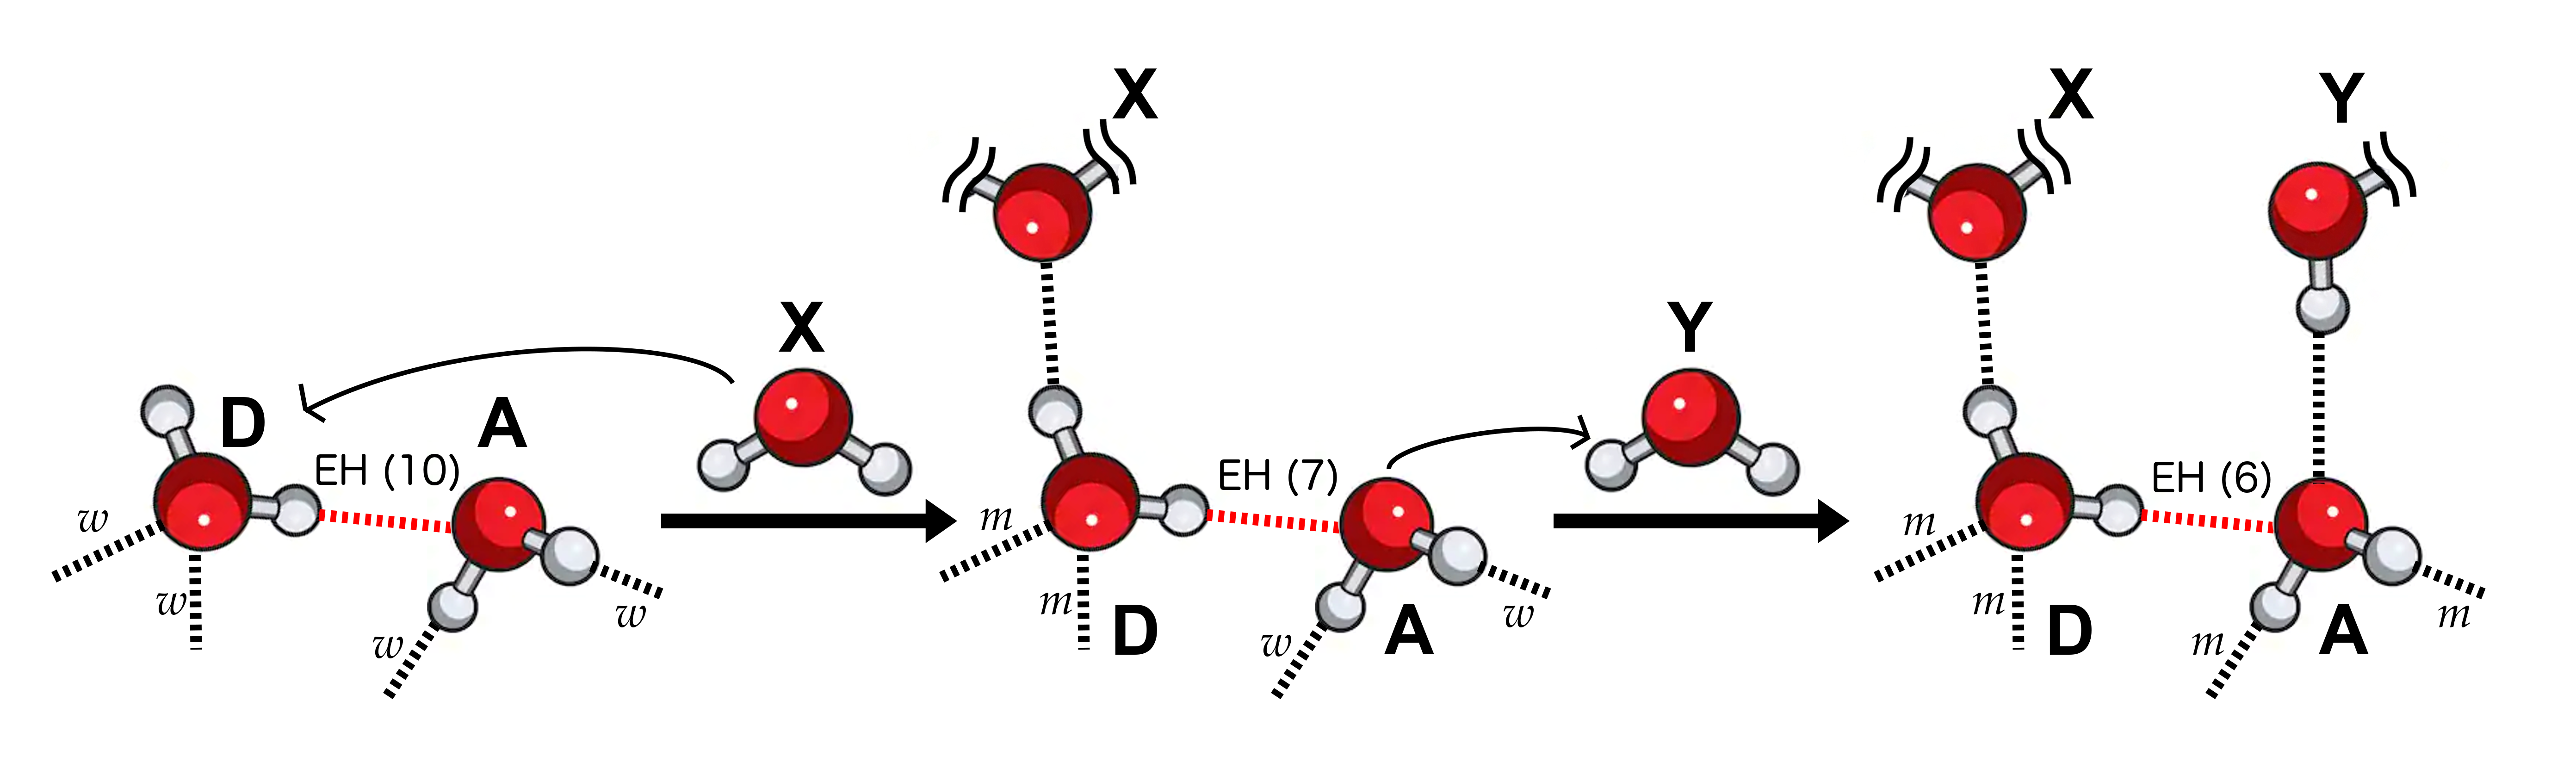
\includegraphics[width=0.86\textwidth]{4/img/figura7}
    \caption{Transición del EH más fuerte (10) al EH tipo (7) y finalmente al tipo (6), a través de donar y aceptar EHs.}
\label{transicion_}
\end{figure}
%La razón detrás de la disparidad en la energía de los diferentes tipos de EH
%radica en como la carga es redistribuida en la formación de cada interacción.
%Cuando un EH es formado, una transferencia de densidad electrónica ocurre del
%EH aceptor al EH donador. La Figura \ref{transferencia} representa el proceso para el
%dimero de agua. Esta transferencia hace que el hidrógeno libre de la molécula
%donante sea un poco menos ácida, obstaculizando la habilidad de esta molécula
%para donar otro protón. Pero por otro lado este mismo desplazamiento de la
%densidad electrónica hacia la molécula aceptora mejora la habilidad del
%correspondiente oxígeno para formar otro EH.
%
%\begin{figure}%{l}{0.45\textwidth}
%    \centering
%    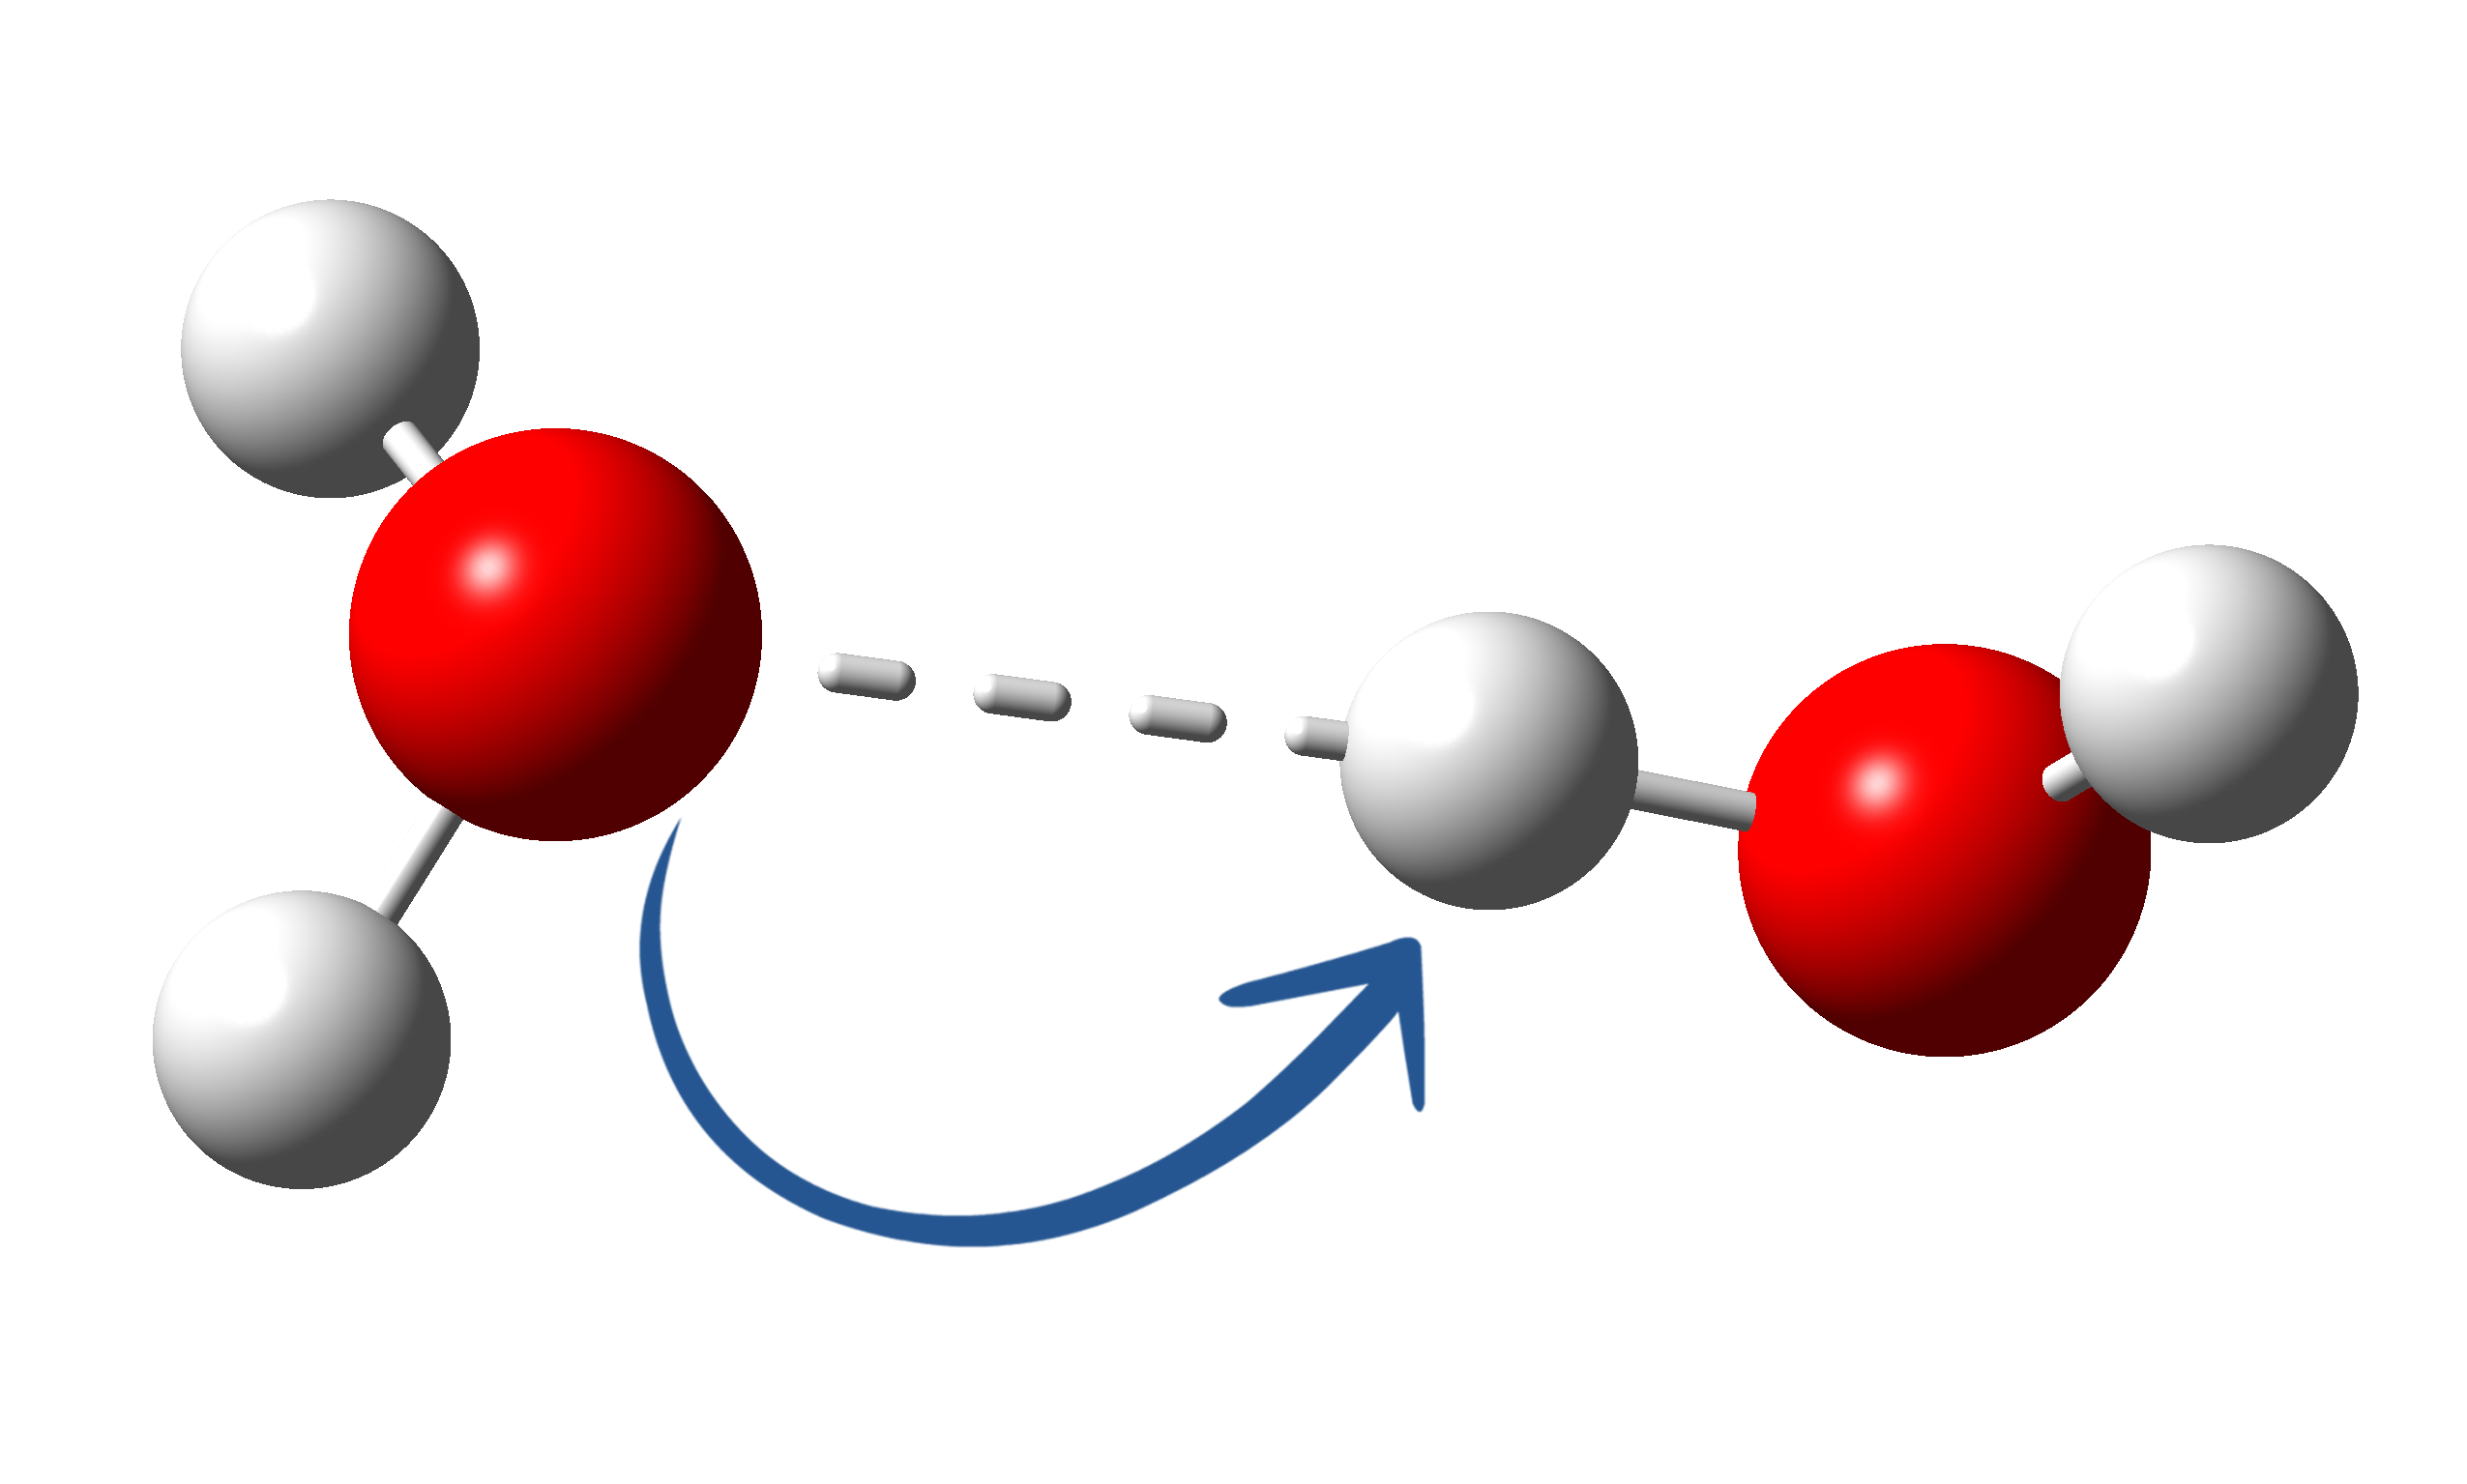
\includegraphics[width=0.55\textwidth]{4/img/dimero_flecha}
%    \caption{Transferencia de densidad elctrónica}
%\label{transferencia}
%\end{figure}
%
%
%
%Siguiendo la misma lógica, podemos ver como una molécula que act'ua como
%un doble donador de EH posee $\rho$ adicional con la que puede participar
%como un buen aceptor de protón en un EH. En forma opuesta, una molécula
%que act'ua como un doble donador de EH tiene una deficiencia de $\rho$, por
%lo que tiene un hidrógeno más ácido y por lo tanto capaz de formar un
%EH más fuerte. Esto corresponde el caso (10) en la Tabla \ref{scale2020}.
%\\
%\section{Descomposición de la energía de interacción entre
%moléculas de agua: e\-ner\-gías clásica y de intercambio}
\section{Distancias Intermoleculares}
%
Usualmente, la energía de interacción y la distancia entre las moléculas están
muy correlacionadas, la Figura \ref{Distances_O-O_new_scale} muestra el
promedio de las distancias entre átomos de oxígeno en función del tipo de EH
reportado en la Tabla \ref{scale2020}. La comparación entre las Figuras
\ref{Distances_O-O_new_scale} y \ref{2016_vs_2020} nos lleva a concluir que
entre mayor sea la distancia promedio entre oxígenos es más débil es la
interacción entre las moléculas.

\begin{wrapfigure}{r}{0.55\textwidth}
    \centering
    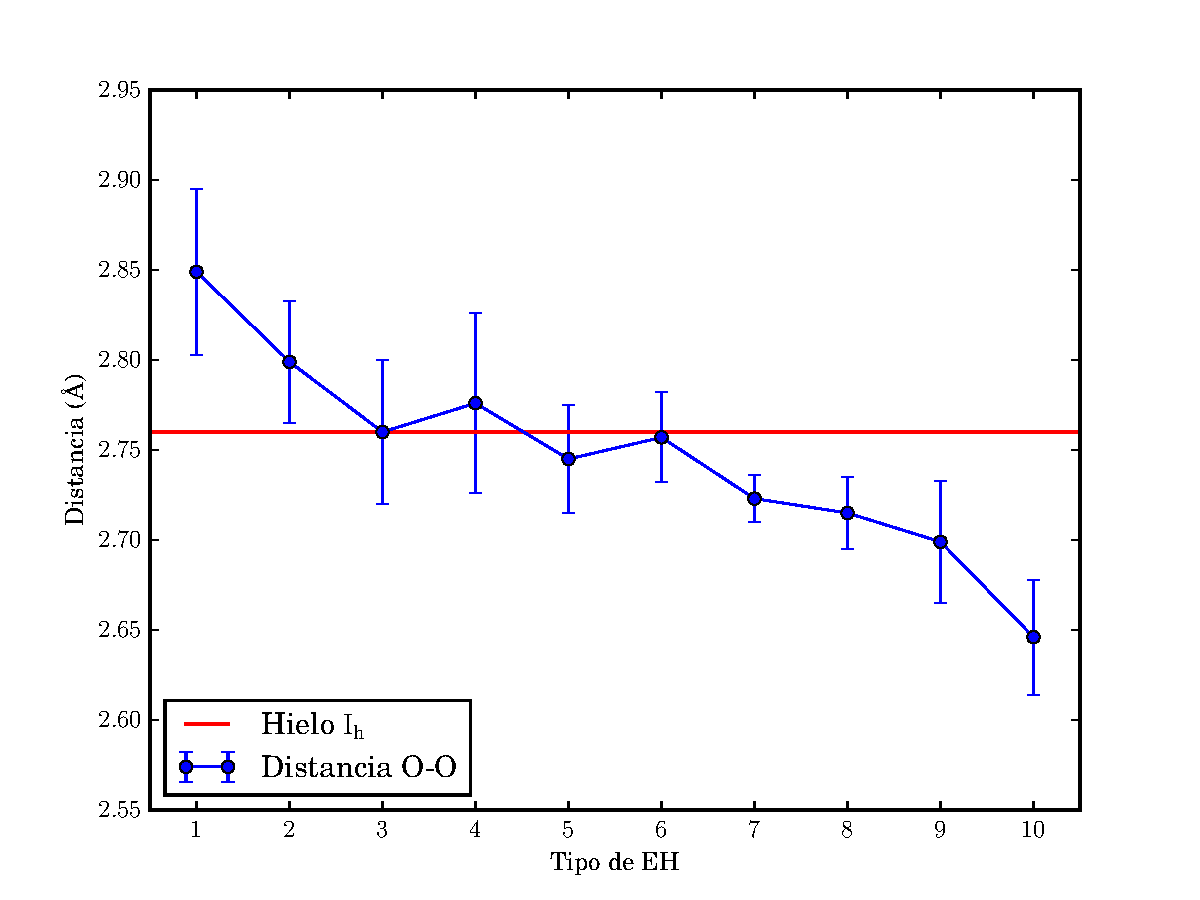
\includegraphics[width=0.60\textwidth]{4/img/Distances_O-O_new_scale}
    \caption{Distancias oxígeno-oxígeno en función del tipo de EH.}
\label{Distances_O-O_new_scale}
\end{wrapfigure}

En la Figura \ref{Distances_O-O_new_scale} se muestra, con una línea roja, la
distancia experimental entre oxígenos reportada para el hielo
$\mathrm{I_{h}}$~\cite{schulson}. Como podemos observar, el valor es muy
similar a las distancias entre oxígenos presentes en los EHs de media la
escala, es decir, los tipos (3), (4), (5) y (6). Cabe señalar que la distancia
entre oxígenos en el hielo $\mathrm{I_{h}}$ es muy similar a la que se presenta
en el EH del tipo (6), tipo de EH que corresponde con la in\-te\-rac\-ción
entre dos moléculas de agua tetracoordinadas, como la que se presenta en el
estado sólido del hielo $\mathrm{I_{h}}$.

\section{Estimación de la Energía de Enlace en Hielo I$\mathrm{_{h}}$}

Usando los valores de energía de interacción es posible estimar la energía
asociada con el proceso de ruptura de los EHs dentro de un mol de hielo
$\mathrm{I_{h}}$, es decir la sublimación:
%
\begin{align}
\mathrm{H_2O_{(s)}} \rightleftharpoons \mathrm{H_2O_{(g)}}.
\end{align}

Para esto, consideramos la energía de interacción entre dos moléculas de agua
en el hielo como el valor correspondiente a la energía de EH del tipo (6) en la
nueva escala reportada en la Tabla \ref{scale2020}, en donde ambas moléculas
son tetracoordinadas, y tiene un valor de \SI{-7.36}{\kilo \calorie \per
\mole}. Cada molécula de agua en el hielo forma cuatro EHs, pero si
consideramos cuatro EHs por molécula, estaríamos contando el doble debido a que
cada EH está formado por dos moléculas, por lo tanto la energía correspondiente
a romper todas las interacciones intermoleculares en un mol de hielo es dos
veces el promedio de energía de interacción entre dos moléculas de agua,
\SI{14.72}{\kilo \calorie \per \mole}. Si comparamos este resultado con el
valor reportado para la entalpía de sublimación, $\Delta H_\mathrm{sub}$,
extrapolado a 0 K \SI{11.38}{\kilo \calorie \per \mole}~\cite{Feistel2007}
vemos que la metodología logra reproducir el valor de la energía de sublimación
con un error de \SI{3.34}{\kilo \calorie \per \mole}.

\section{Componentes Iónicas y Covalentes en la ${E_{\mathrm{int}}^{\mathrm{H_2O}\cdots\mathrm{H_2O}^{ \, \prime}}}$}

En el esquema de partición energética de IQA es posible dividir la energía de
interacción en sus componentes clásicas, o iónicas, y el de
intercambio-correlación, o covalentes. En la Figura \ref{cl_xc} se muestran los
valores correspondientes a estas contribuciones a la energía de interacción
entre las moléculas de agua para los distintos tipos de EHs en la escala de la
Tabla \ref{scale2020}. Podemos observar como los valores para el término
clásico, $V_{\mathrm{cl}}^{\ce{H2O}\cdots\ce{H2O}^{ \, \prime}}$, son algo
similares para todos los tipos de EHs en esta clasificación. Por el contrario,
la energía de intercambio-correlación,
$V_{\mathrm{xc}}^{\ce{H2O}\cdots\ce{H2O}^{ \, \prime}}$, tiene una clara
dependencia con tipo de EH.  Por lo que podemos afirmar que las variaciones en
la energía de interacción provienen, principalmente, del término de
intercambio-correlación.


En la Figura \ref{DI} se muestra el promedio de los valores de DIs entre las
moléculas de agua de los diferentes tipo de EHs. Los DIs, de igual forma que el
término de intercambio-correlación, es una medida de la covalencia de la
interacción entre las moléculas de agua. Los EHs con las mayores energías de
formación tienen mayor cantidad de densidad electrónica compartida y, por lo
tanto, de covalencia.  Esto se refleja en los valores de
DI$^{\ce{H2O\bond{...}H2O}}$ y
$V_{\mathrm{xc}}^{\ce{H2O\bond{...}H2O^{\prime}}}$. De hecho, existe una fuerte
correlación entre las cantidades mencionadas, tal como se observa en la Figura
\ref{XC_vs_di}. Dicha correlación puede ser explotada debido a que el costo
computacional para el cálculo de DI representa sólo una fracción del
correspondiente a la de la $V_{\mathrm{xc}}^{\ce{H2O}\cdots\ce{H2O}^{ \,
\prime}}$.

\begin{figure}[h]
    \centering
    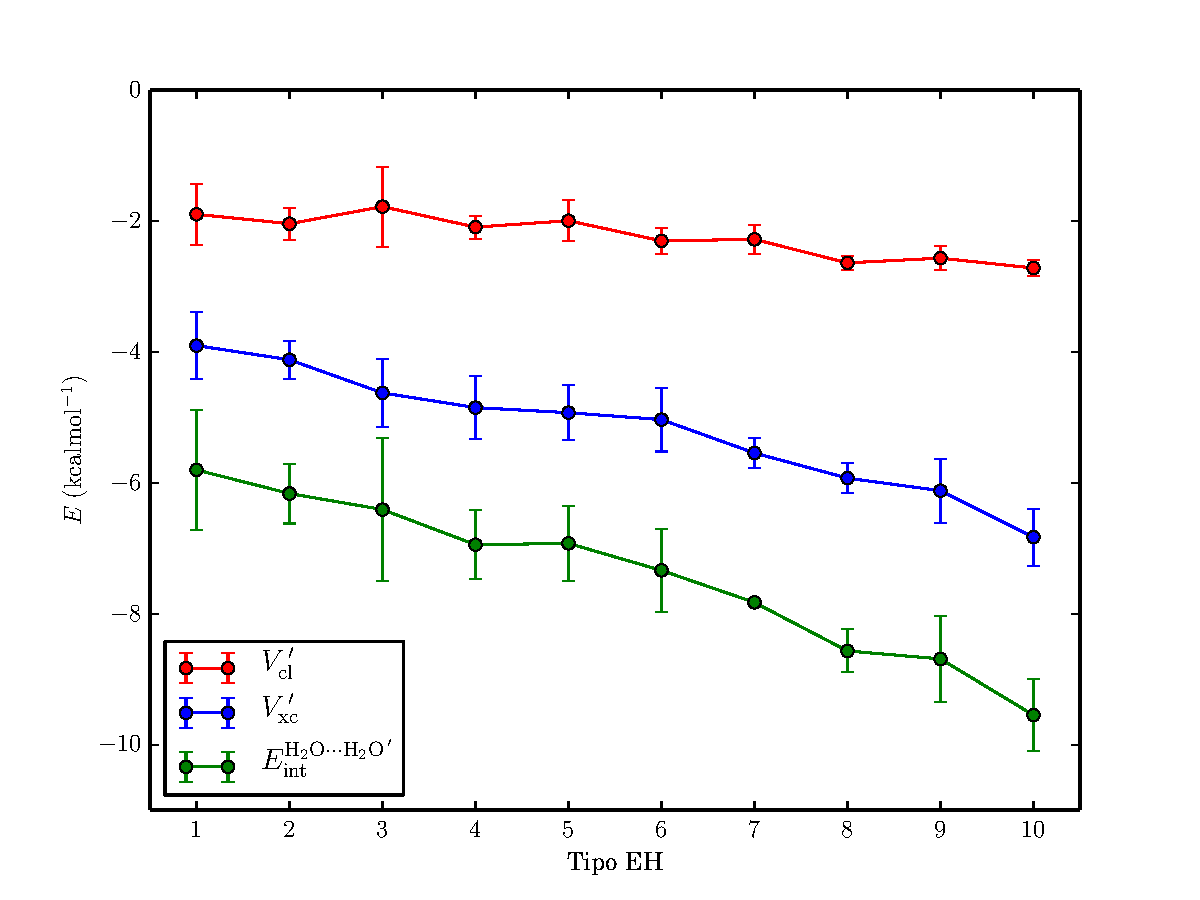
\includegraphics[width=0.70\textwidth]{4/img/Cl_XC}
    \caption{Contribuciones clásicas y de intercambio-correlación.}
\label{cl_xc}
\end{figure}
%
\begin{figure}[h]
    \begin{minipage}[t]{0.50\textwidth}
      \centering
      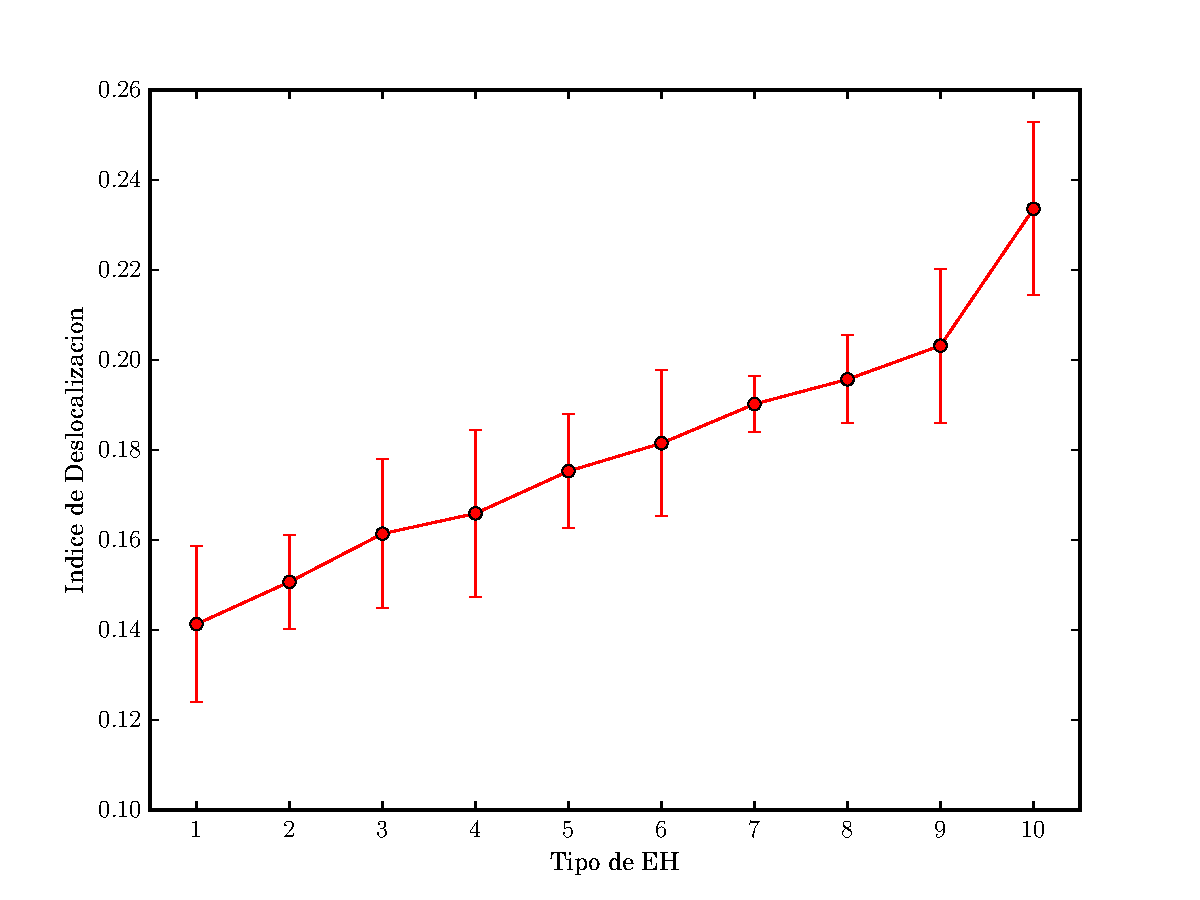
\includegraphics[width=\textwidth]{4/img/DI}
      \caption{Índice de deslocalización \\(unidades atómicas).}
      \label{DI}
    \end{minipage}%
    \hfill
    \begin{minipage}[t]{0.50\textwidth}
      \centering
      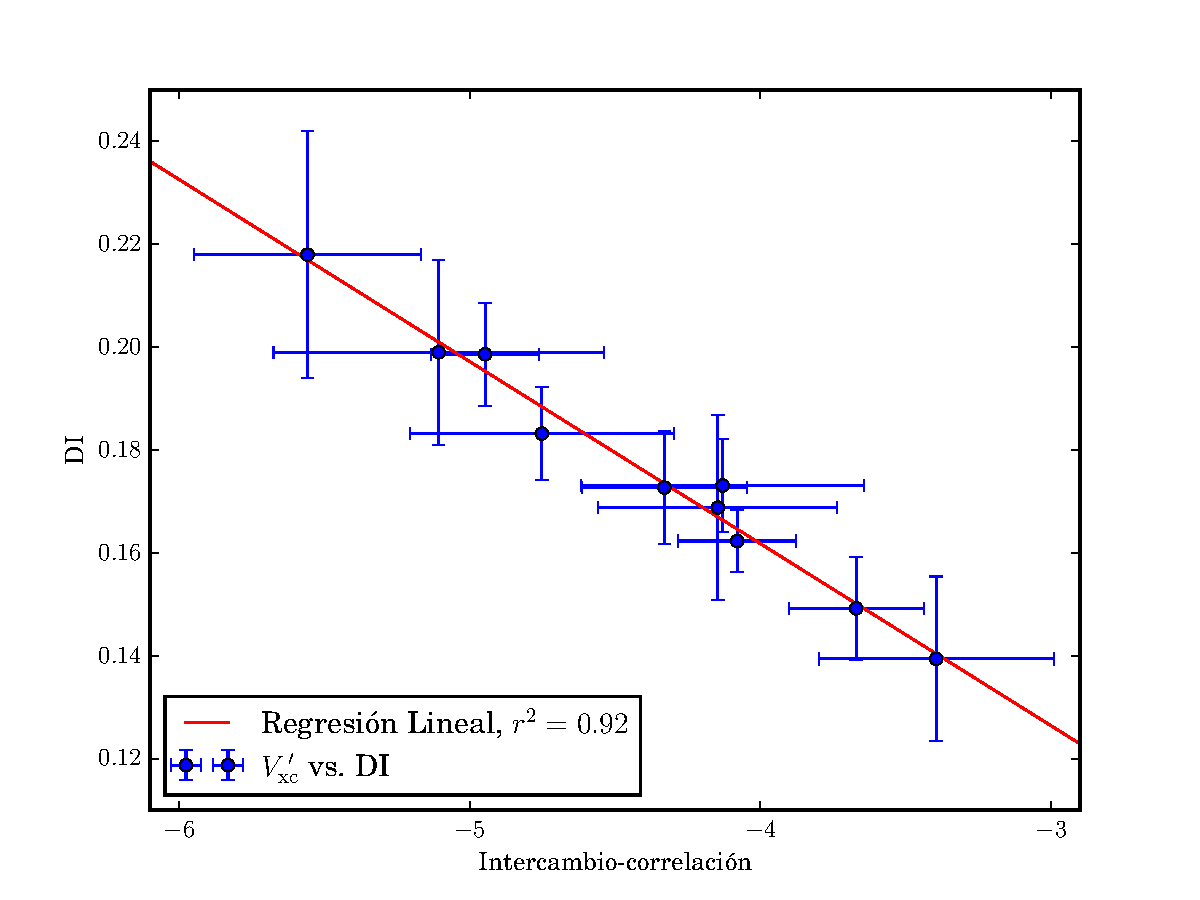
\includegraphics[width=\textwidth]{4/img/XC_vs_di}
      \caption{Regresión lineal entre DI$^{\ce{H2O\bond{...}H2O}}$ (unidades atómicas) y $V_{\mathrm{xc}}^{\ce{H2O\bond{...}H2O^{\prime}}}$ (\SI{}{\kilo \calorie \per \mole}).}
      \label{XC_vs_di}
    \end{minipage}%
\end{figure}

%\newpage
%\thispagestyle{empty}

